\documentclass[a4paper]{article}

%% Page Size and Margins
\usepackage[a4paper,top=3cm,bottom=2cm,left=2cm,right=2cm,marginparwidth=1.75cm]{geometry}

%% Useful packages
\usepackage{graphicx}
\usepackage{fancyhdr}
\usepackage{hyperref}

%%\usepackage{amsmath}
%%\usepackage[colorinlistoftodos]{todonotes}
%%\usepackage[colorlinks=true, allcolors=blue]{hyperref}
%%\usepackage{caption}
%%\usepackage{subcaption}
%%\usepackage{sectsty}
%%\usepackage{apacite}
%%\usepackage{float}
%%\usepackage{titling} 
%%\usepackage{blindtext}
%%\usepackage[square,sort,comma,numbers]{natbib}
%%\usepackage[colorinlistoftodos]{todonotes}
%%\usepackage{xcolor}
%%\definecolor{darkgreen}{rgb}{0.0, 0.4, 0.0}

%% Document Begin
\begin{document}

%% titlepage
\begin{titlepage}
\vspace*{100px}
\newcommand{\HRule}{\rule{\linewidth}{0.5mm}} 	
\center 
 
% Fisrt row
{ \huge \bfseries SerialProxy}
\vspace*{50px}

% Program info
\HRule \\[0.8cm]

\textsc{\normalsize \emph {Simple program for displaying serial communication}}\\[0.8cm]

\HRule \\[1cm]

%%Picture
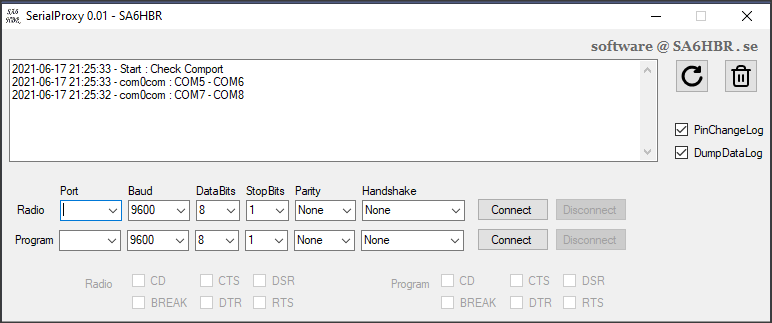
\includegraphics[width=0.6\textwidth]{../image/SerialProxy.png}\\[3cm] 

{\large \today}\\[2cm]
\textsc{ \huge \bfseries SA6HBR}\\[1cm]

\vfill 
\end{titlepage}

\pagestyle{fancy}
\fancyhf{}
\lhead{\today}
\rhead{SA6HBR}

%%\lhead{Guides and tutorials}
\cfoot{ \thepage}

%% Section English
%%\section*{English}

%%Simple program for displaying serial communication
%%\newpage

%% Section Svenska
\section*{Svenska}

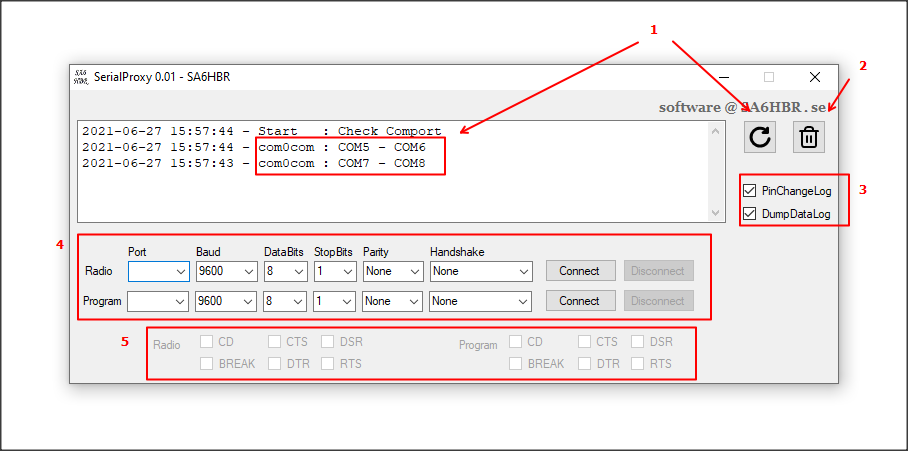
\includegraphics[width=1\textwidth]{../image/SerialProxyInfo.png}\\[1cm] 


\begin{enumerate}   
\item Refresh för komportar. Uppdaterar rullistorna och skriver ut datorns komportar och com0com-paren i loggrutan. 
\item Tömmer loggrutan
\item Väljer vad som skall loggas
\item Inställningr för komportar
\item Visar status för komportarnas in och utgångar
\end{enumerate}  

\vspace*{50px}

\includegraphics[width=0.8\textwidth]{../image/Diagram1.png}\\[1cm] 
Normal inkoppling är att radion kopplas direkt till programmet och programmet som annars kopplas till radion, kopplas nu till ett komportspar.
\newline
Komportspar kan skapas med hjälp av com0com.


\newpage

%% Section  Useful Links
\section*{Useful Links}

* Null-modem emulator (com0com) \href{https://sourceforge.net/projects/com0com/}{https://sourceforge.net/projects/com0com/}. 

%% Section License
\section*{License}

GNU General Public License v3.0


\end{document}